\documentclass[pre,preprint,superscriptaddress]{revtex4-1} 

\usepackage{graphicx}
\usepackage{hyperref}
\usepackage{amsmath}
\usepackage{amsfonts} % needed for bold Greek, Fraktur, and blackboard bold
\usepackage{amssymb}
\usepackage[margin=1in]{geometry}
\usepackage{dcolumn}
\usepackage{multirow}
\usepackage{tikz}
\usetikzlibrary{calc,patterns,decorations.pathmorphing,decorations.markings}
\usepackage{hyperref}
\usepackage{float}
\usepackage{subfig}
\usepackage{todonotes}
\usepackage{subfiles}

% TODO: remove these lines, which expand the margins (useful for comments)
\textwidth  .72\paperwidth
\hoffset -1in
\oddsidemargin .14\paperwidth
\evensidemargin .14\paperwidth
\marginparwidth .11\paperwidth


% Draft macros
\usepackage[normalem]{ulem} % for strikethrough
%\usepackage[usenames,dvipsnames]{xcolor}
%\newcommand{\TODO}[1]{\marginpar{\raggedright\scriptsize\textbf{TODO:} #1} (\textbf{TODO})}
%\newcommand{\NOTEMARG}[1]{\marginpar{\raggedright\scriptsize\textbf{NOTE:} #1} (\textbf{NOTE})}
%\newcommand{\NOTE}[1]{\marginpar{\footnotesize\textbf{NOTE}} (\textbf{NOTE: #1})}
%\definecolor{purple}{rgb}{1,0,1}


\newcommand{\eq}[1]{eq.~\eqref{eq:#1}}
\newcommand{\eqs}[2]{eqs.~\eqref{eq:#1} and \eqref{eq:#2}}
\renewcommand{\sec}[1]{section~\ref{sec:#1}}
\newcommand{\secs}[2]{sections~\ref{sec:#1} and \ref{sec:#2}}
\newcommand{\subsec}[1]{section~\ref{subsec:#1}}
\newcommand{\subsubsec}[1]{section~\ref{subsubsec:#1}}
\newcommand{\app}[1]{appendix~\ref{app:#1}}
\newcommand{\fig}[1]{figure~\ref{fig:#1}}
\newcommand{\figs}[2]{figures~\ref{fig:#1} and \ref{fig:#2}}
\newcommand{\tab}[1]{table~\ref{tab:#1}}
\newcommand{\nn}{\nonumber}




\begin{document}

\title{Time dependent forcing in the Swift Hohenberg equation}
\author{Punit Gandhi}
 \email{punit_gandhi@berkeley.edu}
\author{C\'edric Beaume}
\author{Edgar Knobloch}
 \email{knobloch@berkeley.edu}
\affiliation{Department of Physics, University of California, Berkeley CA 94720, USA}
\date{\today}

\begin{abstract}
The Swift Hohenberg equation has a stable attracting periodic solution for sufficiently strong forcing which does not exist for weak forcings.  When the bifurcation creating this solution from the trivial state is subcritical, there also exists a region of bistability where both the periodic state and the trivial state coexist and are stable.  There also exists a pinning region where an infinite snake of stable localized solutions exist in addition to the periodic and trivial states.   We add a time-periodic forcing to the Swift Hohenberg equation that takes the system between these regions of parameter space.  For specific values of the frequency, amplitude, and center of the periodic forcing, we (hopefully) find something interesting.
\end{abstract}

\maketitle

\section{Introduction}
The Swift-Hohenberg equation (SHE) serves as a model for pattern formation in a broad range of physical systems.   This equation, which takes the form  
\begin{equation}
u_t= r u-\left(1+\partial_{x}^2\right)^2u+N[u]\label{eq:SH},
\end{equation}
describes the dynamics of a real field $u$ over one spatial dimension in time, where $N$ is some nonlinear function of $u$.  We have rescaled the equation so that the critical wavenumber that defines the natural wavelength of the patterned state is unity.  We will be interested in two possible choices of $N$, namely $N_{23}[u]=bu^2-u^3$ and $N_{35}[u]=b u^3-u^5$.  The strength of the linear forcing term $r$ and the strength of the quadratic nonlinearity $b$ are left as parameters of the system.  

We consider the case when the forcing is no longer constant in time, namely $r\rightarrow r_0+\delta r \sin\omega t$.  Pattern formation in ecological systems that are periodically forced by the seasons or the daily variations in insolar flux are one example of a physical motivation for considering this kind of system \cite{}.  Other physical systems that might be described by such a periodically forced model include ... \cite{}.   Furthermore, oscillations that effectively create and destroy attractors have been shown to produce new ``ghost" attractors that do not exist in the time-independent system for any value of the parameter\cite{}.  While this has been done for the case of simple oscillators, it would be interesting to find the analogous dynamics for more complicated pde systems that oscillate between states.

We first recount the relevant details of the original Swift-Hohenberg equation before discussing some numerical results of the time-dependent forced case.  Hopefully we will also eventually add a section describing some theoretical understanding of the results we obtained.  Note that all the work done so far is for the $N_{23}$ nonlinearity and $b=1.8$.


\section{bistability and localized solutions in the SHE}
Here we will describe the structure of the steady-state solutions of SHE near the bifurcation that creates the periodic state.  We will focus on the case when the nonlinearity parameter $b$ creates these states in a subcritical bifurcation from the trivial state at $r=0$.  A bifurcation diagram of the steady state solutions (Fig.~\ref{fig:BurkeSHE}, from J. Burke et et al) shows the trivial state, the periodic state, and localized solution branches.  

\begin{figure}[h]\center
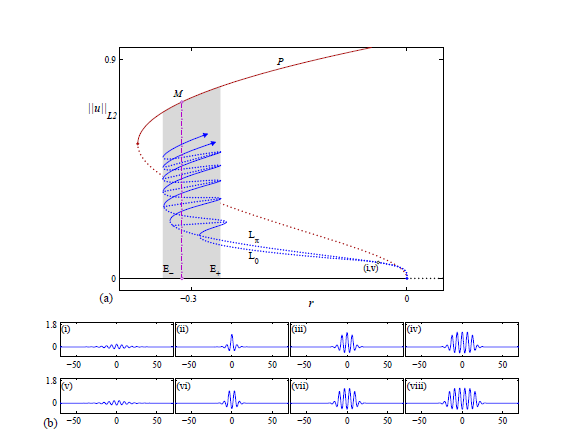
\includegraphics[width=120mm]{BurkeSHE.PNG}
\caption{\label{fig:BurkeSHE}This figure was taken from Burke\cite{} (a) Bifurcation diagram showing the snakes-and-ladders structure of localized states. Away from the origin the snaking branches $L_0$ and $L_-$ are contained within the snaking region (shaded) between$E_-$ and $E_+$, where $r(E_-)\approx -0.3390$ and $r(E_+)\approx -0.2593$.   Solid (dotted) lines indicate stable (unstable) states. In addition, the Maxwell point $M$, occurring at $r(M)\approx -0.3128$  is indicated with a vertical dash-dot line (b) Sample localized profiles $u(x): (i-iv)$ lie on $L_0$, near onset and at the 1st, 3rd, and 5th saddle-nodes from the bottom, respectively; (v-viii) lie on $L_-$, near onset and at the 1st, 3rd, and 5th saddle-nodes, respectively. Parameters: $b = 1.8$.}
\end{figure}

We see that the trivial solution is stable for $r<0$, and becomes unstable as as the periodic solution is created through a bifurcation at $r=0$.  As we are looking at the subcritical case, we see a saddle-node bifurcation of the periodic branch where it gains stability at $SN_P$.  Thus we have only a stable trivial solution for $r<r(SN_P)\approx -0.3744$. At this point, a stable periodic solution is created but is energetically unfavorable to the trivial state.  For $r(E_-)<r<r(E_+)$, we have a zoo of localized solutions (including an entire sequence of stable localized solutions on each snaking branch) that exist in addition to trivial and periodic solutions.  We note that within this region, $r(M)$ indicates the transition from the trivial state being energetically favorable to the periodic state becoming energetically favorable.  We will also find it useful to define the center of the snaking region $C$, which corresponds to  the forcing parameter $r(C)\approx -0.2992$.  Between $r(E_+)$ and $r=0$, we again have only the periodic solution and the trivial solution as stable but with the periodic solution now more energetically favorable.   Finally, for $r>0$, the trivial solution looses stability and only the periodic solution remains as stable.  We note that other stable solutions exist (e.g. the flat, nonzero solutions created at the transcritical bifurcation at $r=1$) but that they do not play a role in our region of interest with our current choice of parameters (e.g. $b=1.8$).  {\it I plan eventually replace J. Burke's figure with one that clearly indicates these different regions}.

In addition to understanding the structure of the stationary solutions, it will also be helpful to understand what is known about the dynamics of the localized solutions when the system is pushed just outside of the snaking region.  Burke and Knobloch \cite{} have shown that near the snaking region (e.g. for $r=r(E_{\pm})\pm\delta$ where $\delta <<1$), a localized solution will move towards the more energetically favorable of the trivial and the periodic state.  Above the snaking region, for example, a localized solution will nucleate periods of the pattern in quick bursts with some longer transition time $T\propto \delta^{-1/2}$ in between each nucleation event.  An numerical example of this using the method of exponential differencing \cite{} to step in time and a domain of 40 periods of the characteristic wavelength is shown in Fig.~\ref{fig:nucleation}.  A localized solution that is stable for $r\approx 0.2944$ is initialized above the snaking region (e.g. $r=0.2$) and allowed to grow until it fills the domain. We note that it grows to a solution containing 39 periods, and a corresponding numerical continuation calculation produces a snaking branch of steady state solutions that emerges as a secondary bifurcation from a 40 period solution by reconnects to a 39 period solution.  This phenomena has been explained \cite{} in terms of the Eckhaus instability for the case of the steady state solutions.  We can see from Fig.~\ref{fig:nucleation} that the time from one nucleation event to the next is approximately 18, though the last nucleation event seems to take a bit longer.  As the transition time $T$ for this case is on the same order as the time over which the nucleation event occurs, we have likely reached the limit of applicability of the theory described above.

\begin{figure}[h]
  \begin{center}
    \mbox{
      \subfloat[]{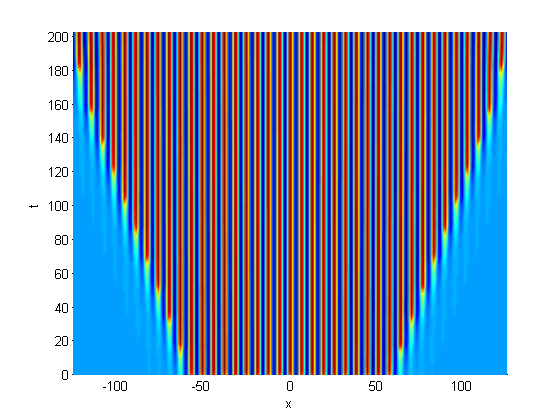
\includegraphics[width=60mm]{NucleationSolution.png}} \quad
      \subfloat[]{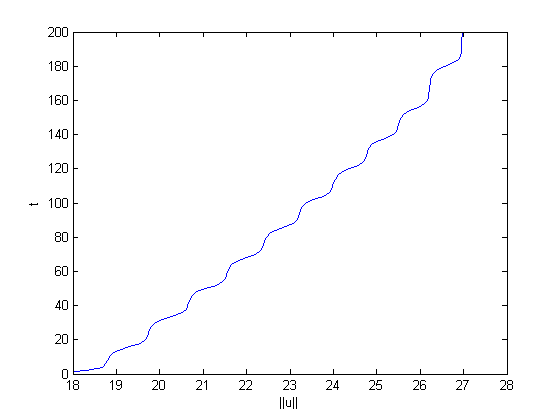
\includegraphics[width=60mm]{NucleationNorm.png} }
      }
    \caption{A simulation of the SHE with $N_{23}$, $b=1.8$ and $r=-0.20$ (e.g. $\delta\approx 0.06$) is initialized using a localized solution that is stable within the snaking region (e.g. at $r=-0.2944$). The solution growing in time (a) with red as high values and blue as low values.  The norm of the solution as it grows in time is shown in (b).}
    \label{fig:nucleation}
  \end{center}
\end{figure} 

\section{Numerical results}

All simulations in time used periodic boundary conditions and a domain of $80\pi$ (e.g. 40 characteristic wavelengths).  A 4th order exponential time differencing scheme\cite{} was used to step forward  in time while spectral methods on a grid of 1024 points were used for the spatial calculations.  The  calculation of steady state solutions were done by numerical continuation using AUTO~\cite{}.   We will focus on SHE23 case with $b=1.8$ and will always initialize the problem with a stable localized solution that fills roughly half the domain.  We can vary the way the forcing oscillates ($r\rightarrow r_0+\delta r \sin\omega t$) in 3 ways: (1) the amplitude of the oscillation, $\delta r$ (2) the point about which the oscillation occurs, $r_0$ (3) the frequency with which the oscillation occurs, $\omega$.

The phase space of this problem is infinite dimensional, but can choose a two dimensional slice of the max value vs L2 norm of u to help us visualize trajectories in time.  All the plots will also contain the periodic and snaking branch of the time steady solutions (Fig.~\ref{fig:NormMaxBack}) as reference.  

\begin{figure}[h]
  \begin{center}
    \mbox{
      \subfloat[]{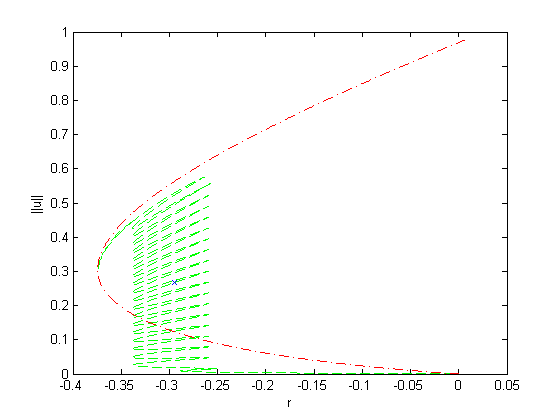
\includegraphics[width=60mm]{NormrBack.png}} \quad
      \subfloat[]{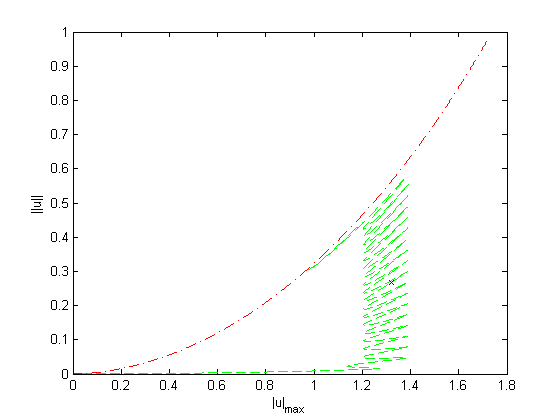
\includegraphics[width=60mm]{NormMaxBack.png} }
      }
    \caption{(a)A plot of the time-steady localized (green dash) and periodic (red dash-dot) solutions as a function of the forcing parameter in the problem with constant $r$ in time.  The blue x indicates the localized initial solution for the simulations with time-periodic forcing.  We note that future plots will zoom into the region near this x.  (b) This same data is plotted in terms of the max value vs L2 norm of the solutions in order to provide some reference for the trajectories of the time-dependent parameter case. }
    \label{fig:NormMaxBack}
  \end{center}
\end{figure} 

We first oscillate the forcing about the Maxwell point within the snaking region for various frequencies of oscillation.  We note that the time scale on which the nucleation process occurs is 10


\bibliography{TimeForcingSHE_bibliography}

\end{document}
